\documentclass[aspectratio=169,10pt]{beamer}
\usepackage[T1]{fontenc}
\usepackage[utf8]{inputenc}
\usepackage[brazil]{babel}
\usepackage{lmodern}
\usepackage{amsmath,amssymb,booktabs,graphicx}
\usetheme{Madrid}
\definecolor{navy}{RGB}{22,50,79}
\definecolor{teal}{RGB}{8,126,139}
\setbeamercolor{structure}{fg=navy}
\setbeamercolor{frametitle}{bg=navy,fg=white}
\setbeamercolor{block title}{bg=teal,fg=white}
\setbeamertemplate{navigation symbols}{}
\setbeamertemplate{footline}[frame number]
\setbeamertemplate{itemize items}[circle]
\graphicspath{{assets/}}
\setbeameroption{hide notes}
\title{MLP do zero para MNIST}
\subtitle{Fundamentos de redes neurais com Python e NumPy}
\author{MLP-from-Scratch colaboradores}
\date{15 de novembro de 2026}
\begin{document}
\begin{frame}\titlepage\end{frame}
\section{Parte 1: Fundamentos de redes neurais}
\begin{frame}{Parte 1: Fundamentos de redes neurais}
\tableofcontents[currentsection]\end{frame}

\begin{frame}{Por que implementamos uma MLP}
\begin{itemize}
\item Queríamos conectar matrizes e derivadas a um sistema que aprende.
\item Implementamos cada operação de aprendizado em Python e NumPy.
\item Nosso objetivo é uma referência educacional reprodutível, sem reivindicar o estado da arte.
\end{itemize}
\end{frame}

\begin{frame}{O que é uma rede neural?}
\[f_{\theta}(x)=W_L^{\top}\,\phi(\cdots\phi(W_1^{\top}x+b_1)\cdots)+b_L\]\begin{itemize}
\item Uma função parametrizada que transforma entradas em saídas.
\item Camadas combinam evidências; ativações não lineares tornam a composição expressiva.
\item No aprendizado supervisionado, exemplos rotulados orientam a atualização dos parâmetros.
\end{itemize}

\note{A expressão ilustra vetores-coluna; nossa implementação armazena exemplos nas linhas.}
\end{frame}

\begin{frame}{Neurônios biológicos e artificiais}
\begin{tabular}{p{.43\textwidth}p{.48\textwidth}}\toprule Neurônio biológico & Neurônio artificial\\\midrule Dendritos recebem sinais & Entradas contêm atributos numéricos\\[6pt] Sinapses influenciam a transmissão & Pesos multiplicam cada entrada\\[6pt] Dinâmica celular produz atividade elétrica & Uma ativação transforma uma soma ponderada\\\bottomrule\end{tabular}\par\vspace{10pt}Essa é uma analogia, não uma simulação fiel do cérebro.\end{frame}

\begin{frame}{Pesos e vieses}
\[z=\sum_{j=1}^{d}w_jx_j+b,\qquad a=\phi(z)\]\begin{itemize}
\item Um peso controla a contribuição de uma entrada; seu sinal pode favorecer ou contrariar a resposta.
\item O viés desloca a resposta mesmo quando as entradas são zero.
\item Aprendemos pesos e vieses; escolhemos taxa de aprendizado e arquitetura como hiperparâmetros.
\end{itemize}
\[x=(0.2,0.8),\quad w=(0.5,-0.25),\quad b=0.2\quad\Rightarrow\quad z=0.1\]\end{frame}

\begin{frame}{Ativação ReLU}
\[\operatorname{ReLU}(z)=\max(0,z),\qquad \operatorname{ReLU}^{\prime}(z)=\mathbf{1}_{z>0}\]\begin{itemize}
\item Valores positivos passam; valores negativos viram zero.
\item Sem ativações não lineares, camadas afins empilhadas equivalem a uma única transformação afim.
\item Definimos derivada zero na origem e usamos inicialização de He nas camadas escondidas.
\end{itemize}
\[W_{ij}\sim\mathcal{N}(0,2/n_{\mathrm{in}}),\qquad b=0\]\end{frame}

\begin{frame}{Nossa arquitetura}
\[784\;\longrightarrow\;128\;\longrightarrow\;64\;\longrightarrow\;10\]\begin{itemize}
\item Duas camadas densas escondidas com ReLU; a saída linear retorna dez logits.
\item 109.386 parâmetros treináveis, incluindo vieses.
\item Os pesos da saída usam Xavier; os pesos escondidos usam He.
\end{itemize}
\[(784\cdot128+128)+(128\cdot64+64)+(64\cdot10+10)=109386\]\end{frame}

\begin{frame}{Propagação direta de um lote}
\[Z^{(\ell)}=A^{(\ell-1)}W^{(\ell)}+b^{(\ell)}\]\[X\in\mathbb{R}^{B\times784}\to A^{(1)}\in\mathbb{R}^{B\times128}\to A^{(2)}\in\mathbb{R}^{B\times64}\to Z^{(3)}\in\mathbb{R}^{B\times10}\]\begin{itemize}
\item Cada linha é uma imagem; a multiplicação de matrizes processa o lote em conjunto.
\item O treino guarda entradas e máscaras ReLU para a retropropagação.
\end{itemize}
\end{frame}

\begin{frame}{Softmax e classe prevista}
\[p_{ic}=\frac{\exp(z_{ic}-m_i)}{\sum_k\exp(z_{ik}-m_i)},\qquad m_i=\max_k z_{ik}\]\[\widehat y_i=\operatorname*{arg\,max}_{c}p_{ic}\]\begin{itemize}
\item Subtrair o máximo preserva as probabilidades e evita estouro na exponencial.
\item Os escores somam um; valores altos não garantem acerto nem calibração.
\end{itemize}
\end{frame}

\section{Parte 2: Visão geral do dataset}
\begin{frame}{Parte 2: Visão geral do dataset}
\tableofcontents[currentsection]\end{frame}

\begin{frame}{Dígitos manuscritos do MNIST}
\centering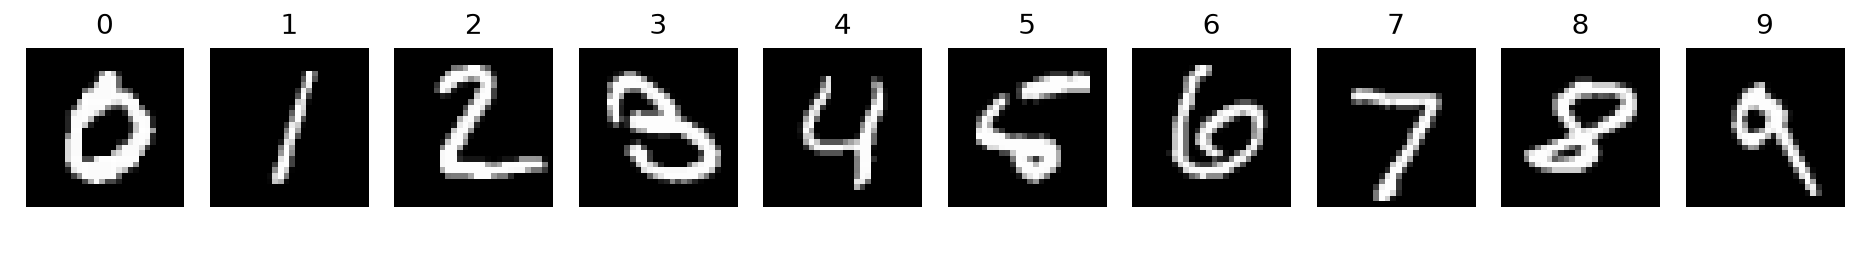
\includegraphics[width=\textwidth]{mnist.png}\par\raggedright\begin{itemize}
\item Dez classes: dígitos de 0 a 9, em imagens em tons de cinza com rótulos conhecidos.
\item As partições originais contêm 60.000 imagens de treino e 10.000 de teste.
\item Verificamos os arquivos baixados e interpretamos o formato IDX.
\end{itemize}
\scriptsize Dataset: LeCun, Cortes e Burges. As imagens são exemplos reais do teste.\end{frame}

\begin{frame}{Achatamento e normalização}
\[28\times28=784,\qquad x_j=\frac{\mathrm{pixel}_j}{255}\in[0,1]\]\begin{itemize}
\item Convertemos os pixels para float32 e lemos as linhas em ordem fixa.
\item As entradas têm formato (N, 784); os rótulos inteiros têm formato (N,).
\item A MLP recebe valores em posições fixas, sem uma operação própria de vizinhança espacial.
\end{itemize}
\end{frame}

\begin{frame}{Treino, validação e teste}
\begin{center}\begin{tabular}{lrl}\toprule Partição & Imagens & Finalidade\\\midrule Treino & 50.000 & Atualizar pesos\\ Validação & 10.000 & Selecionar configurações e modelo\\ Teste oficial & 10.000 & Avaliar após a seleção\\\bottomrule\end{tabular}\end{center}\begin{itemize}
\item Dividimos apenas o treino original, com estratificação e seed 42.
\item Usamos apenas normalização: sem correção de inclinação nem aumento de dados nesta execução.
\end{itemize}
\end{frame}

\section{Parte 3: Aprendizado e resultados}
\begin{frame}{Parte 3: Aprendizado e resultados}
\tableofcontents[currentsection]\end{frame}

\begin{frame}{Perda de entropia cruzada}
\[L=-\frac1B\sum_{i=1}^{B}\sum_{c=0}^{9}Y_{ic}\log p_{ic}\]\begin{itemize}
\item Y representa as classes corretas em one-hot; o carregador mantém rótulos inteiros.
\item Um escore baixo para a classe correta recebe uma penalidade maior.
\item Calculamos a perda diretamente dos logits com log-sum-exp deslocado.
\end{itemize}
\[L_i=\log\sum_k e^{z_{ik}-m_i}-(z_{i,y_i}-m_i)\]\end{frame}

\begin{frame}{Retropropagação e regra da cadeia}
\[\frac{\partial L}{\partial w}=\frac{\partial L}{\partial z}\,\frac{\partial z}{\partial w}\]\[\frac{\partial L}{\partial Z^{(3)}}=\frac{P-Y}{B}\]\begin{itemize}
\item Propagamos os gradientes de trás para frente pela composição das camadas.
\item O gradiente mede sensibilidade local, não um erro independente de cada neurônio.
\item A média pelo lote é aplicada uma única vez, no gradiente da perda.
\end{itemize}
\end{frame}

\begin{frame}{Gradientes de uma camada densa}
\[dW=A_{\mathrm{previous}}^{\top}dZ,\qquad db=\sum_{i=1}^{B}dZ_i\]\[dA_{\mathrm{previous}}=dZ\,W^{\top},\qquad dZ_{\mathrm{ReLU}}=dA\odot\mathbf1_{Z>0}\]\begin{itemize}
\item Os gradientes têm as formas dos parâmetros; o gradiente do viés mantém (1, n-out).
\item Calculamos todos os gradientes antes de atualizar os pesos.
\end{itemize}
\end{frame}

\begin{frame}{SGD com mini-lotes}
\[\theta_{t+1}=\theta_t-\eta\nabla_{\theta}L_{\mathrm{batch}}\]\begin{itemize}
\item Usamos taxa de aprendizado 0,1 e lotes de 64, incluindo o último lote menor.
\item Embaralhamos a ordem do treino a cada época.
\item Uma época é uma passagem completa pelos exemplos de treino.
\item Executamos 20 épocas; a seed 42 controla inicialização, divisão e embaralhamento.
\end{itemize}
\end{frame}

\begin{frame}{Nosso ciclo de treinamento}
\begin{itemize}
\item Para cada lote: propagação direta, perda, retropropagação e atualização SGD.
\item No fim da época: recalculamos métricas de treino e validação ponderadas por amostra.
\item Salvamos o modelo com a menor perda de validação.
\item Congelamos a seleção antes de medir o desempenho no teste oficial.
\end{itemize}
\small\texttt{data/mnist.py} $\to$ \texttt{network.py} $\to$ \texttt{trainer.py} $\to$ \texttt{evaluate.py}\end{frame}

\begin{frame}{Perda e acurácia ao longo do treino}
\centering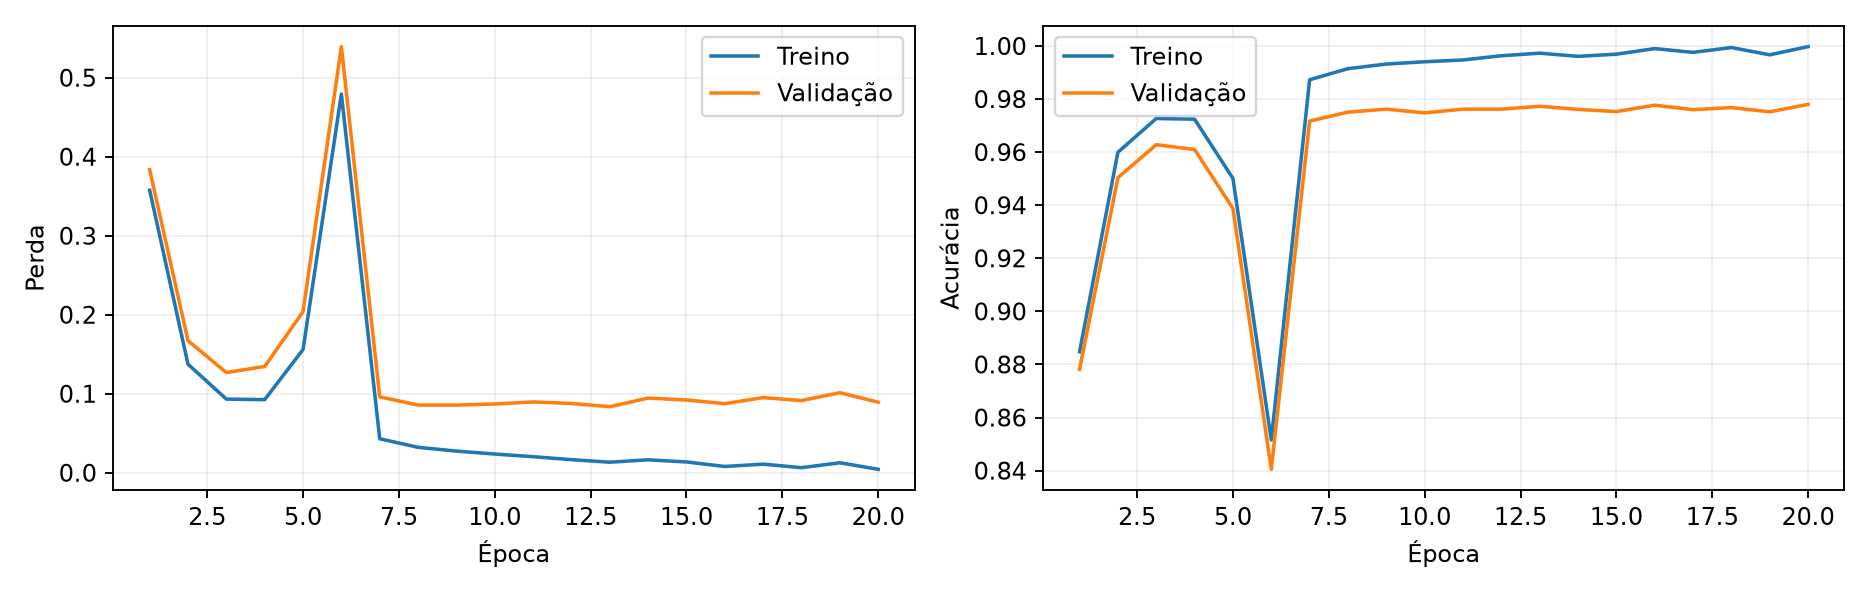
\includegraphics[width=.94\textwidth]{curves_pt.png}\par\raggedright\begin{itemize}
\item A menor perda de validação ocorreu na época 13: 0,083610; acurácia de 97,73\%.
\item Melhorias posteriores no treino não reduziram consistentemente a perda de validação.
\end{itemize}
\end{frame}

\begin{frame}{Avaliação final do modelo selecionado}
\begin{center}\begin{tabular}{lr}\toprule Métrica de teste & Resultado medido\\\midrule Acurácia & 97,90\%\\ Acertos / erros & 9.790 / 210\\ Entropia cruzada & 0,072777\\ Precisão / revocação macro & 97,90\% / 97,87\%\\ F1 macro / ponderado & 97,88\% / 97,90\%\\ ROC AUC macro / micro & 0,999621 / 0,999617\\\bottomrule\end{tabular}\end{center}Uma execução, uma seed, 10.000 imagens oficiais de teste.\par\scriptsize\texttt{results/baseline/extended\_metrics.json}\end{frame}

\begin{frame}{Matriz de confusão}
\begin{columns}[c]\column{.53\textwidth}\centering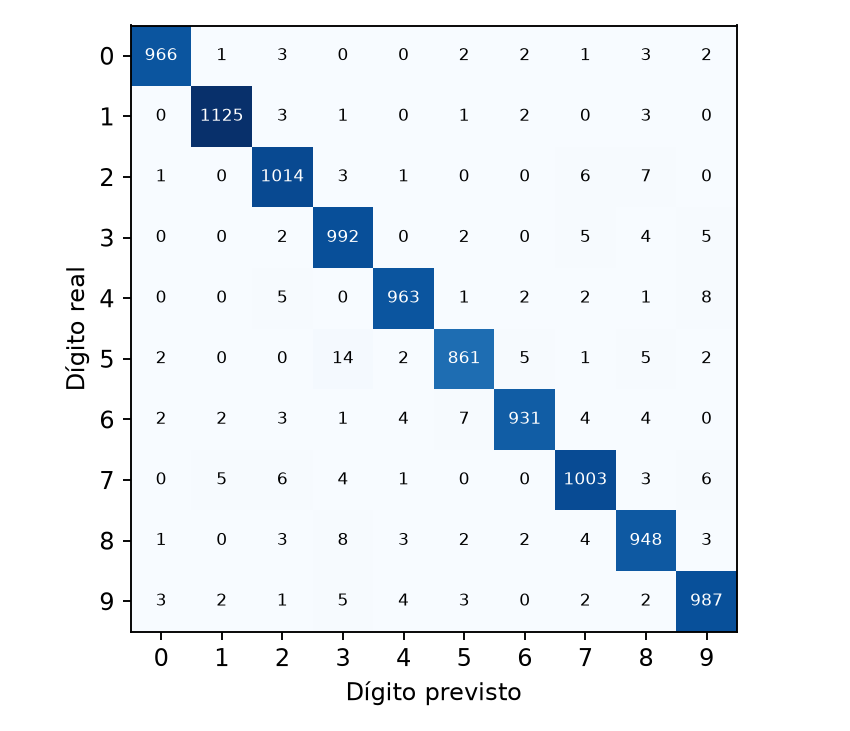
\includegraphics[width=\linewidth,height=.65\textheight,keepaspectratio]{confusion_pt.png}\column{.45\textwidth}\begin{itemize}
\item Linhas são dígitos reais; colunas são previsões.
\item Erro direcionado mais frequente: 5 previsto como 3, com 14 casos.
\item O dígito 8 teve o menor F1: 97,03\%.
\end{itemize}
\end{columns}\end{frame}

\begin{frame}{Curvas ROC e AUC um contra os demais}
\begin{columns}[c]\column{.53\textwidth}\centering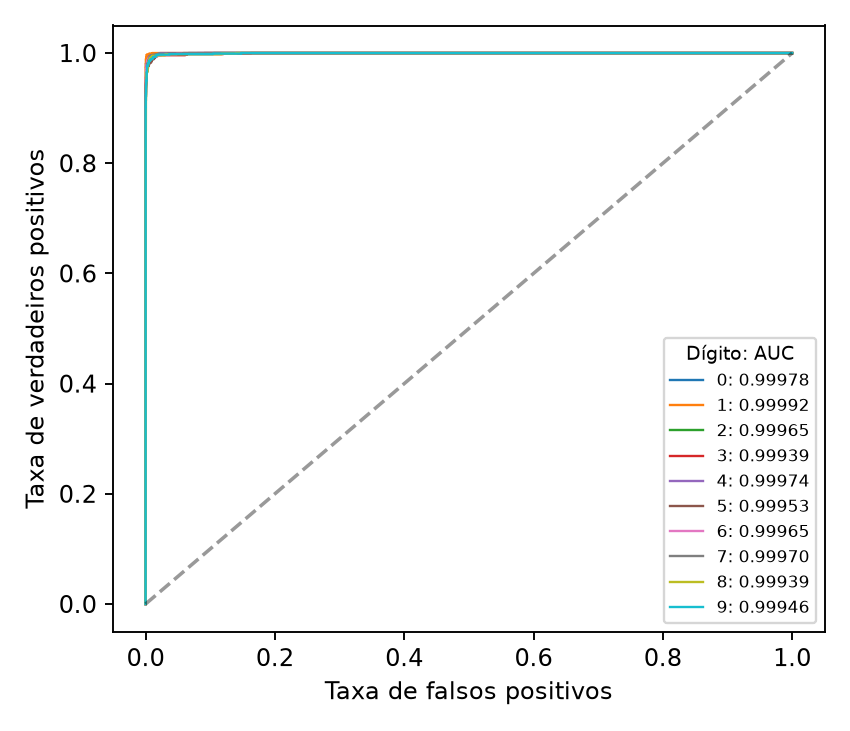
\includegraphics[width=\linewidth,height=.65\textheight,keepaspectratio]{roc_pt.png}\column{.45\textwidth}\begin{itemize}
\item Para cada dígito, variamos um limiar sobre seu escore contra os demais.
\item Macro calcula a média das dez AUCs; micro reúne os pares imagem/classe.
\item AUC alta de ranking não equivale à acurácia multiclasse nem à calibração.
\end{itemize}
\end{columns}\end{frame}

\begin{frame}{Erros reais e previsões confiantes}
\centering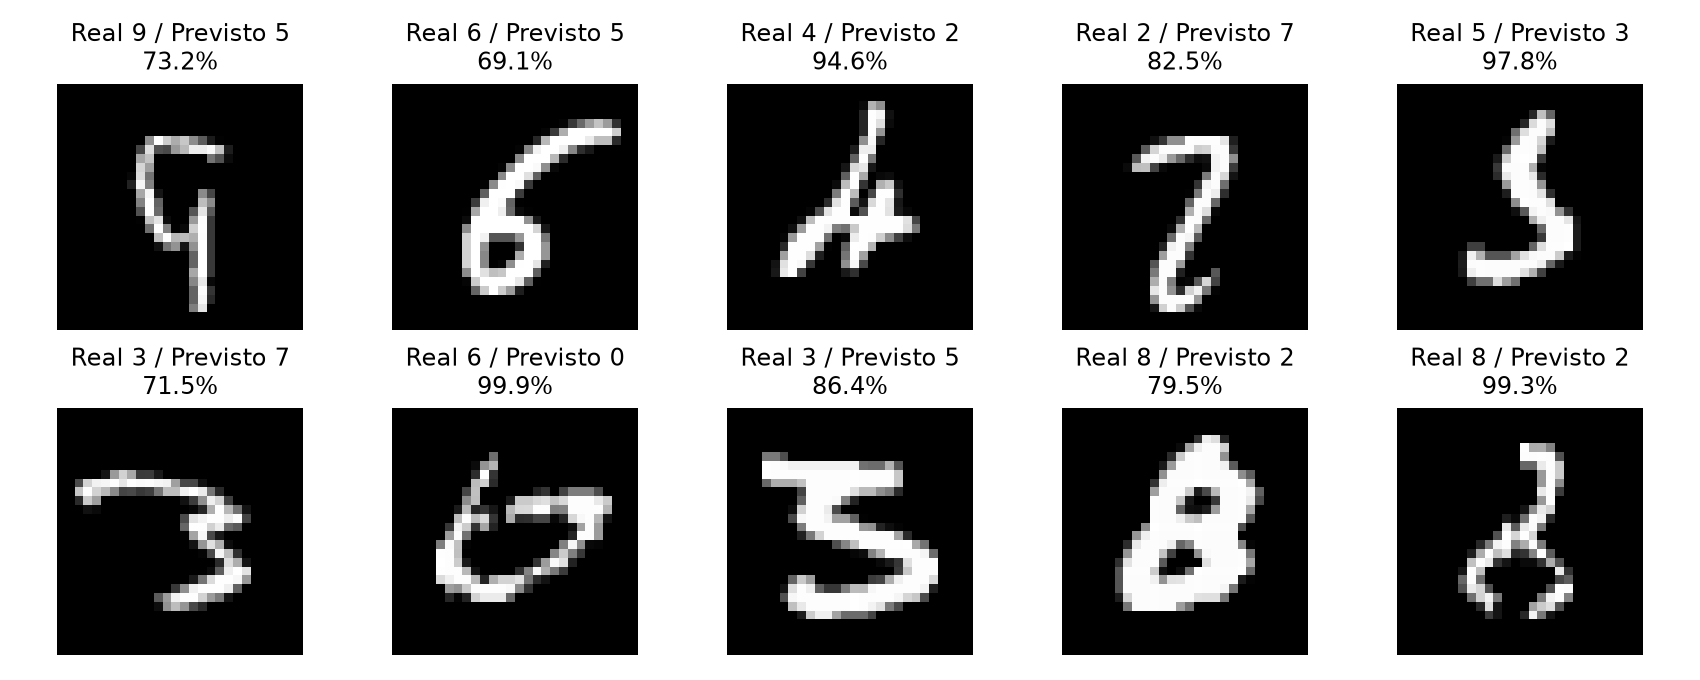
\includegraphics[width=.92\textwidth,height=.61\textheight,keepaspectratio]{errors_pt.png}\par\raggedright Primeiros dez erros na ordem do teste, sem seleção manual. Os valores são escores Softmax da classe prevista.\end{frame}

\begin{frame}{Verificação e limitações}
\begin{itemize}
\item 24 testes cobrem gradientes por diferenças finitas, perda estável, empates na ROC, salvamento e treino.
\item O intervalo de Wilson de 95\% para acurácia é 97,60--98,16\%, sob hipótese binomial, para o modelo fixo.
\item Uma seed não estabelece a variação entre execuções; as saídas Softmax não foram calibradas.
\item Compararíamos seeds, ajustes da taxa e regularização nos dados de validação.
\end{itemize}
\end{frame}

\begin{frame}{O que aprendemos e onde consultar}
\begin{itemize}
\item Conectamos preparação de dados, propagação direta, gradientes e otimização.
\item O resultado é uma evidência reprodutível desta execução, não uma garantia universal de desempenho.
\item Após observar erros do teste, mudanças guiadas por eles precisam de nova evidência reservada.
\end{itemize}
\small\url{https://github.com/jp-tedesco/MLP-from-Scratch}\par\texttt{docs/experiments.md}\quad\texttt{results/baseline/}\par\medskip Referência do dataset: LeCun, Cortes e Burges; espelho CVDF do MNIST. Todos os gráficos usam nosso modelo registrado.\end{frame}

\end{document}
